
\chapter{Graph Neural Networks (GNNs)}

\section{Motivation}
\begin{itemize}
    \item CNNs work well on images
    \item RNNs work well on sequences (one-dimensional)
    \item Both work on Euclidean spaces in $\mathbb{R}^n$
\end{itemize}

\begin{definition}
    \textbf{Non-Euclidean Space:} also known as curved or non-flat spaces, are mathematical spaces that do not follow the rules of Euclidean geometry. They exhibit different geometric properties compared to Euclidean space ($\mathbb{R}^n$), which is flat and follows Euclid's axioms.
\end{definition}

\begin{itemize}
    \item We can use GNNs to model predictions for non-Euclidean spaces (usually graphs).
\end{itemize}

\begin{figure}[h!t]
    \centering
    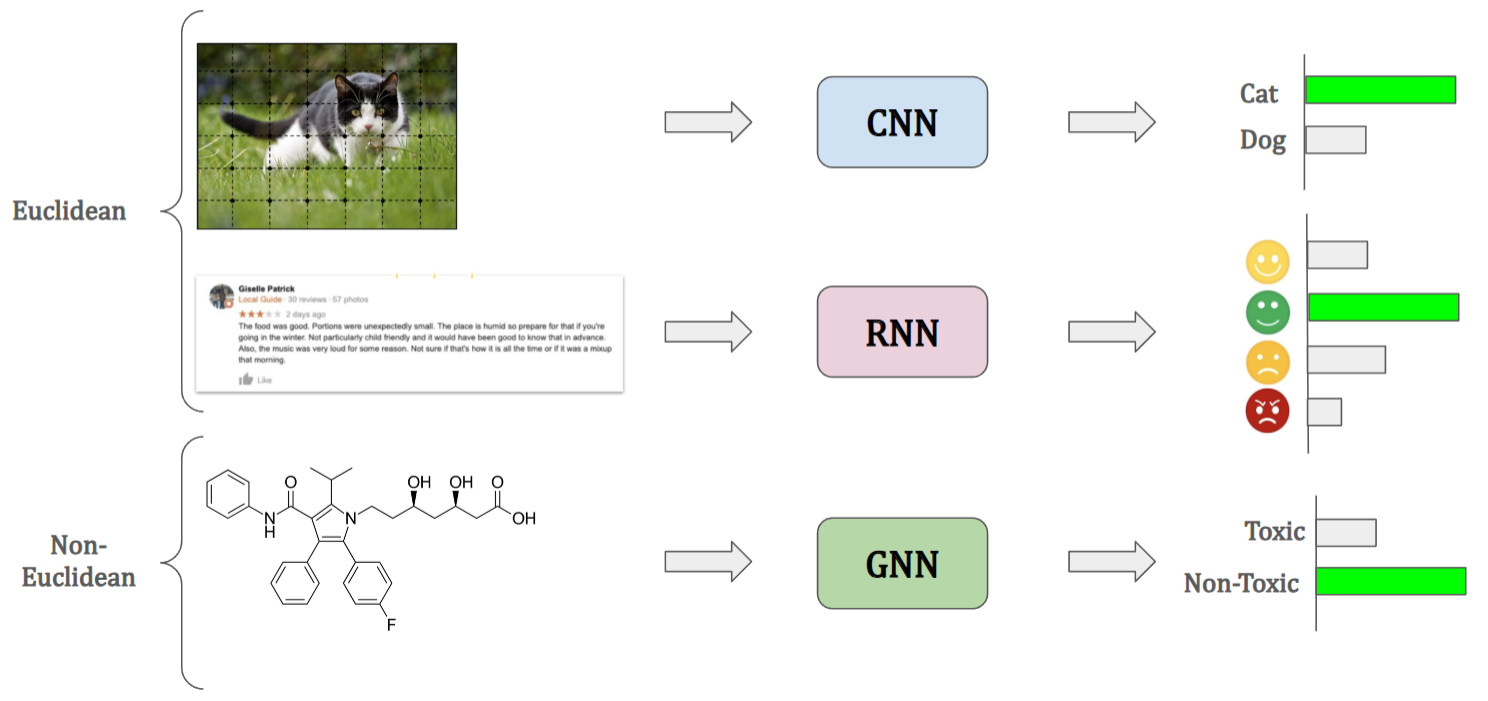
\includegraphics[width=1\linewidth]{gnnsmotivation.png}
    \caption{Why GNNs?}
    \label{fig:enter-label}
\end{figure}

\begin{definition}
    \textbf{Graph:} a mathematical structure consisting of nodes (vertices) and edges (connections) that represent relationships or connections between the nodes.
\end{definition}

\begin{figure}[h!t]
    \centering
    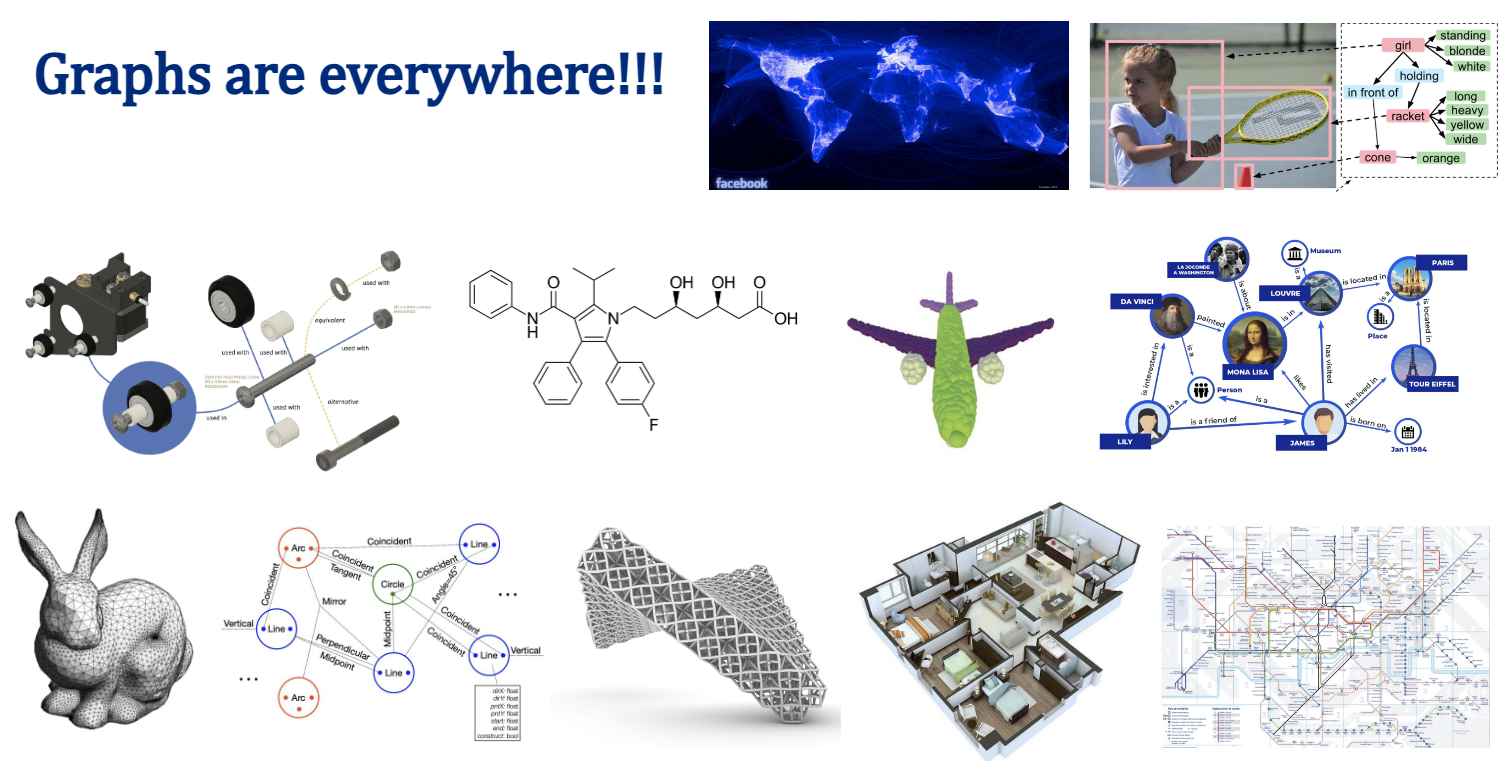
\includegraphics[width=0.75\linewidth]{examplesofgraphs.png}
    \caption{Examples of Graphs}
    \label{fig:enter-label}
\end{figure}

\newpage

\section{Deep Sets}

\noindent
\textbf{Sets}\\
What happens if we \textbf{omit the Positional Encoding} from Transformers?
\begin{itemize}
    \item The input will be treated as a set, and the learned representation won't change if you randomly shuffle the input tokens.
    \item This property is known as \textbf{order-invariance} or \textbf{permutation-invariance}.
    \item But when is this property useful?
\end{itemize}

\begin{figure}[h!t]
    \centering
    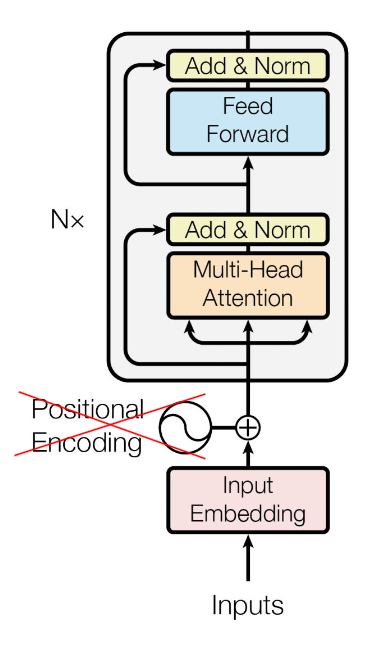
\includegraphics[width=0.25\linewidth]{omitposenc.png}
    \caption{Omitting positional encoding from transformers}
    \label{fig:enter-label}
\end{figure}

Data modalities that we have seen so far have\textbf{ underlying order}. If we shuffle the order of:
\begin{itemize}
    \item Pixels within an image
    \item Words within a sentence
    \item Frames within a video
    \item Signals within audio
\end{itemize}
...they will lose their meaning.\\

What if we want to train a model that predicts the likelihood of a set of items to be purchased by customers in a store?

\begin{figure}[h!t]
    \centering
    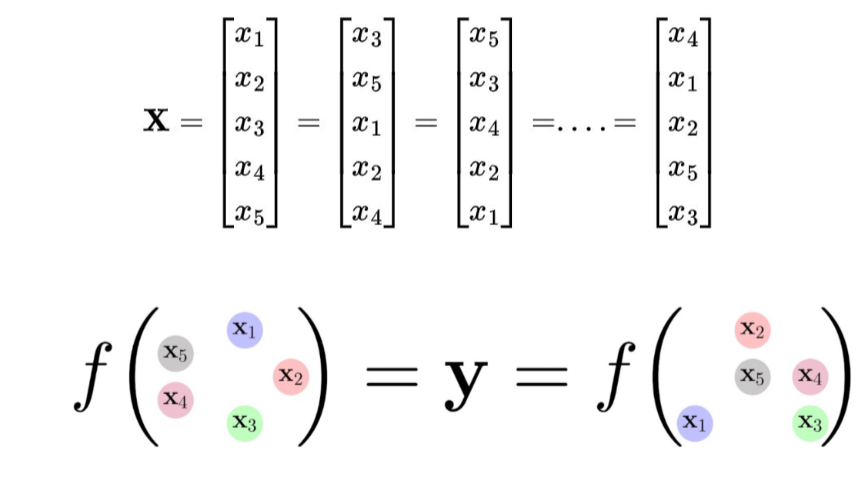
\includegraphics[width=0.5\linewidth]{datainvariance.png}
    \caption{Model must be invariant to the order of the items}
    \label{fig:enter-label}
\end{figure}

\begin{idea}
We want the model to ignore the order in which items are presented because the order is not essential and can confuse the model, similar to how shuffling training data helps prevent the model from learning irrelevant patterns.
\end{idea}
    
\noindent
\textbf{Deep Sets}\\
\begin{enumerate}
    \item Learn embeddings for each item $\rightarrow$ Use a \textbf{shared neural network} $\psi$ (e.g., MLP, Transformer, etc.) to project each item to a shared space.
    \item Learn embeddings for the set $\rightarrow$ Use an \textbf{order-invariant aggregation function} such as sum, mean, max, etc. to aggregate the embeddings into a single embedding.
    \item Use another \textbf{neural network} $\phi$ (e.g., MLP) to project the embedding to the final space.
\end{enumerate}

\begin{figure}[h!t]
    \centering
    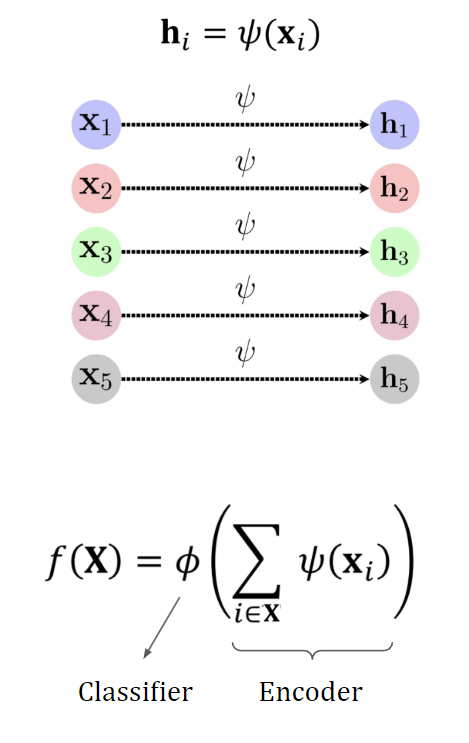
\includegraphics[width=0.275\linewidth]{deepsets.png}
    \caption{Deep Sets}
    \label{fig:enter-label}
\end{figure}

\newpage

\section{Graphs}

Let’s reiterate on Transformers without positional encoding:
\begin{itemize}
    \item The transformer learns an NxN attention matrix which represent pairwise importance scores
    \item This means Transformer creates a fully-connected graph over the input and learns the edge weights
\end{itemize}

\begin{figure}[h!t]
    \centering
    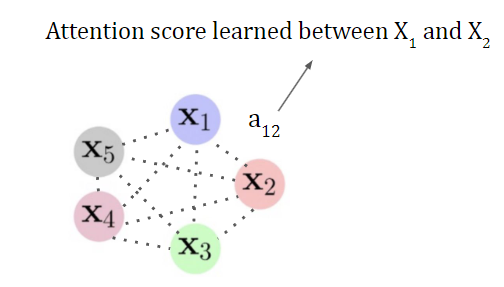
\includegraphics[width=0.75\linewidth]{edgeweights.png}
    \caption{Learning edge weights (attention scores) in a fully-connected graph}
    \label{fig:enter-label}
\end{figure}

\begin{definition}
    \textbf{Graph:}  \textbf{G=(V, E, X)} is a data-structure that encodes \textbf{pair-wise interactions or relations} among \textbf{concepts and objects}:
\begin{itemize}
    \item V is set of nodes representing concepts or objects
    \item $E \subseteq V \times V$ is a set of edges connecting nodes and representing relations or interactions among them
    \item X encodes the node features of each node
    \item We can represent the edges in an \textbf{adjacency matrix} \textbf{A}:
    \item \textbf{Degree} of a node is number of edges connecting to that node
\end{itemize}
\end{definition}

\begin{figure}[h!t]
    \centering
    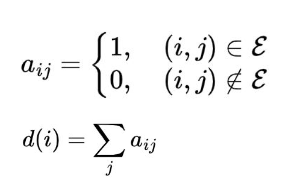
\includegraphics[width=0.4\linewidth]{Adjencymat.png}
    \caption{Adjacency matrix (1 = connection; 0 = no connection)}
    \label{fig:enter-label}
\end{figure}

\begin{figure}[h!t]
    \centering
    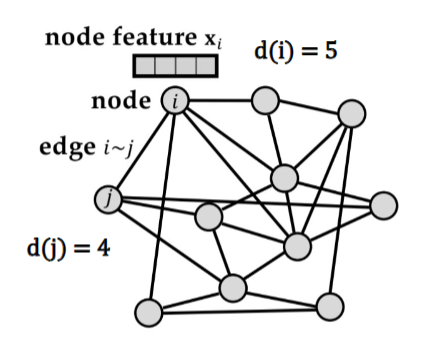
\includegraphics[width=0.35\linewidth]{graph.png}
    \caption{Graph}
    \label{fig:enter-label}
\end{figure}

\begin{itemize}
    \item Graphs are \textbf{order-invariant}: the naming or ordering of nodes may be shuffled and the graph won't change

\begin{figure}[h!t]
    \centering
    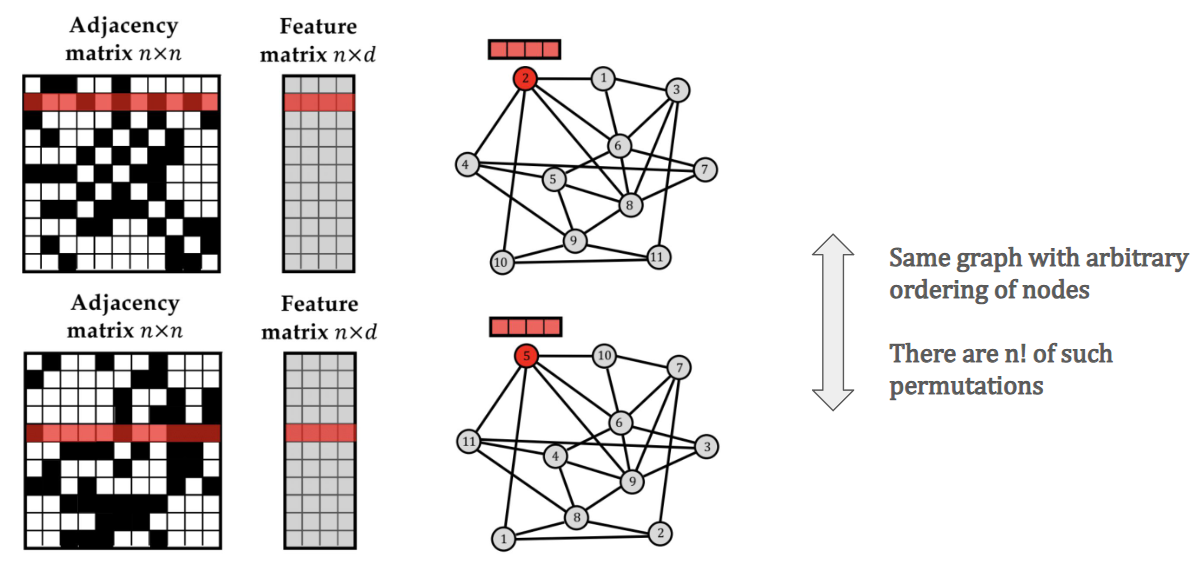
\includegraphics[width=0.75\linewidth]{orderinvarian.png}
    \caption{Indices and naming are arbitrary}
    \label{fig:enter-label}
\end{figure}

    \item Functions on graphs must also be order-invariant
\end{itemize}

\begin{figure}[h!t]
    \centering
    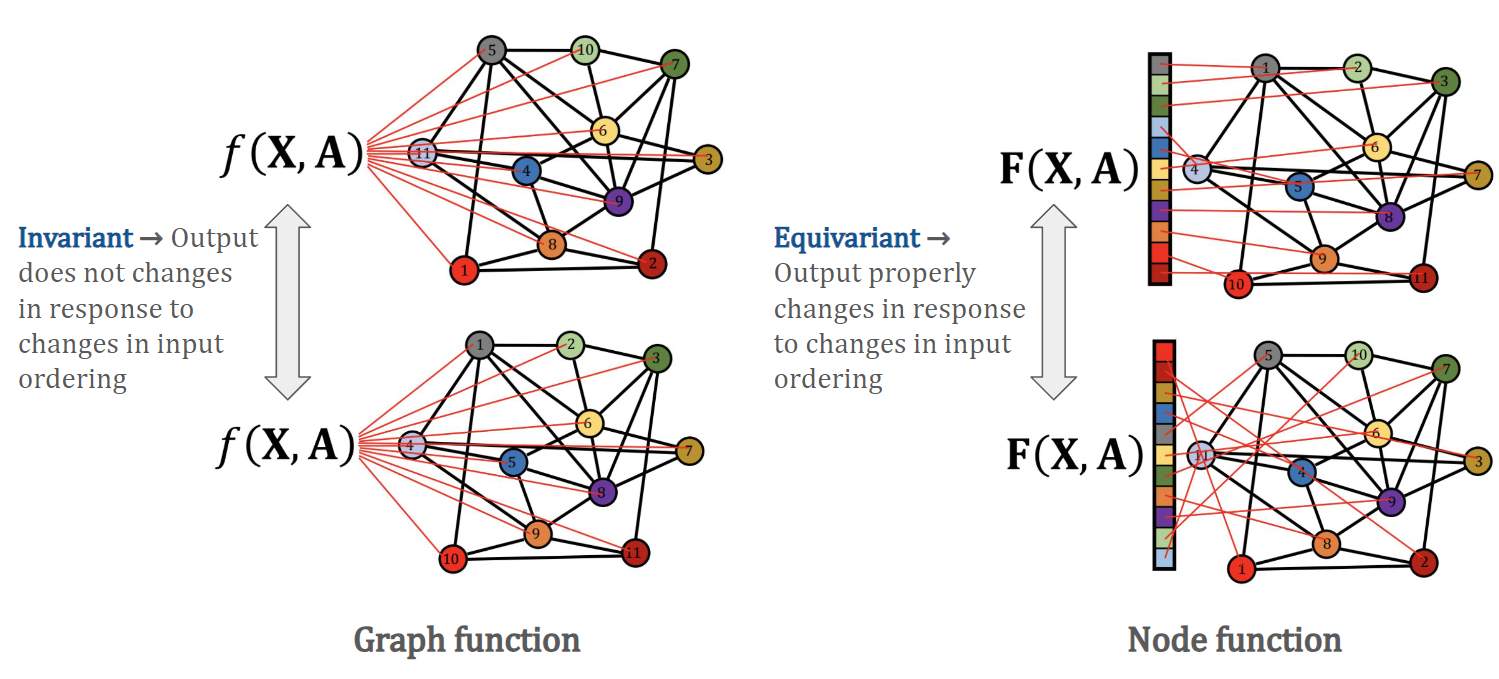
\includegraphics[width=0.75\linewidth]{fnorderinv.png}
    \caption{Invariance and Equivariance}
    \label{fig:enter-label}
\end{figure}


\section{Graph Neural Networks}
\begin{definition}
    \textbf{Graph Neural Networks:} a class of deep learning models specifically designed to work with structured data represented as graphs. The key idea behind GNNs is to extend neural network architectures to handle data with a graph structure, such as social networks, recommendation systems, molecular chemistry, and more.
\end{definition}

\begin{itemize}
    \item GNNs are neural networks that function on graphs
    \item They are mostly based on \textbf{Message-Passing} → communicate with neighbors to update embeddings
    \item \textbf{Node classification}: we can use them to predict node classes
    \begin{itemize}
        \item Eg. Predicting atom types in molecule structure
    \end{itemize}
    \item \textbf{Graph classification}: We can use them to predict graph classes
    \begin{itemize}
        \item Eg. Predicting if a molecule structure is toxic
    \end{itemize}
    \item \textbf{Link prediction}: We can use them to predict links between nodes
    \begin{itemize}
        \item Eg. Predicting if there should be a bond between two atoms
    \end{itemize}
\end{itemize}

\begin{figure}[h!t]
    \centering
    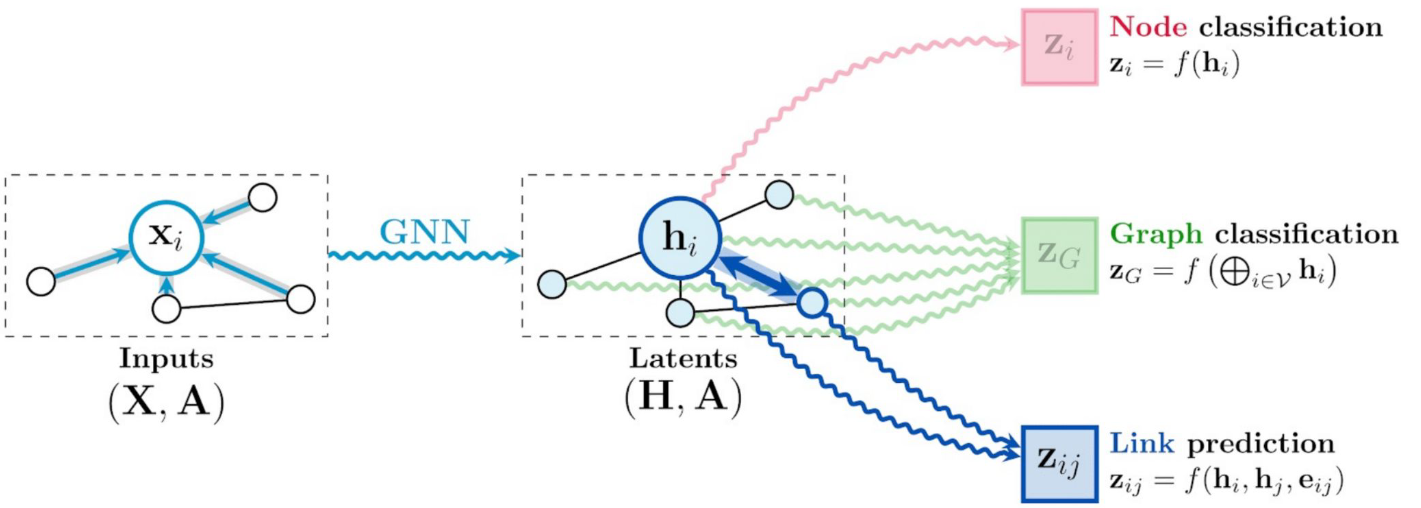
\includegraphics[width=0.65\linewidth]{messagepassing.png}
    \caption{Message passing and application examples}
    \label{fig:enter-label}
\end{figure}

\noindent
\textbf{Message Passing}\\
For each node in graph:
\begin{enumerate}
    \item \textbf{Aggregate} embeddings of its neighbor nodes
    \item \textbf{Combine} the aggregated embedding with the node embedding
    \item  \textbf{Update} the node embedding
\end{enumerate}

\begin{figure}[h!t]
    \centering
    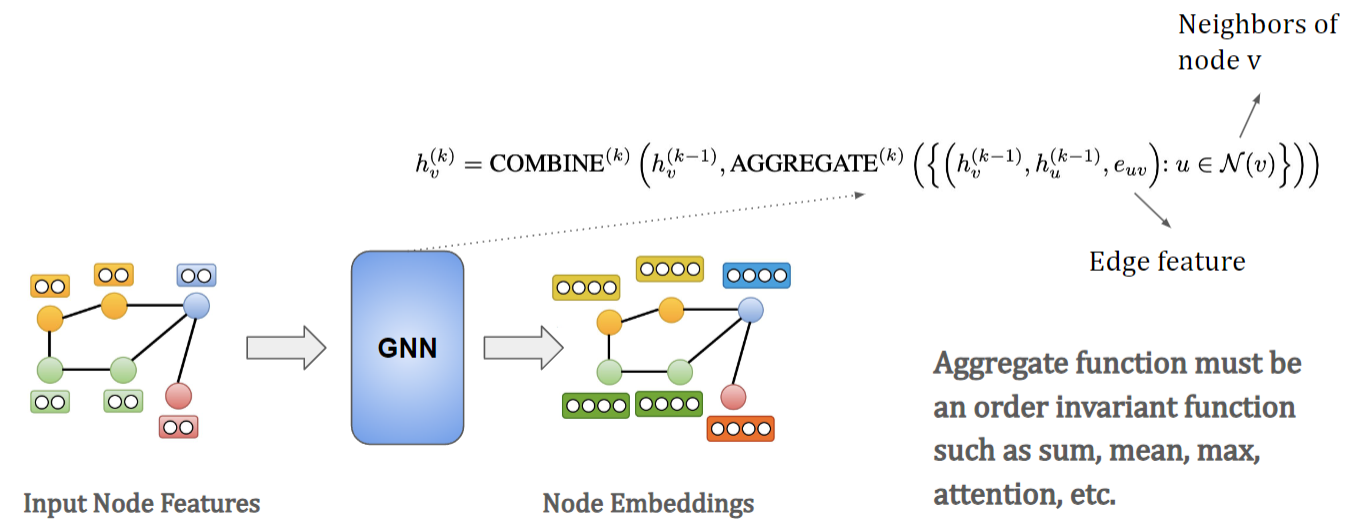
\includegraphics[width=0.75\linewidth]{messagepassingf.png}
    \caption{Message Passing}
    \label{fig:enter-label}
\end{figure}
\newpage

\textbf{Read-out (graph pooling) function}\\
\begin{itemize}
    \item Aggregates all node embeddings into a graph embedding
    \item Must be an order invariant function such as sum, mean, max, attention, etc.
\end{itemize}

\begin{figure}[h!t]
    \centering
    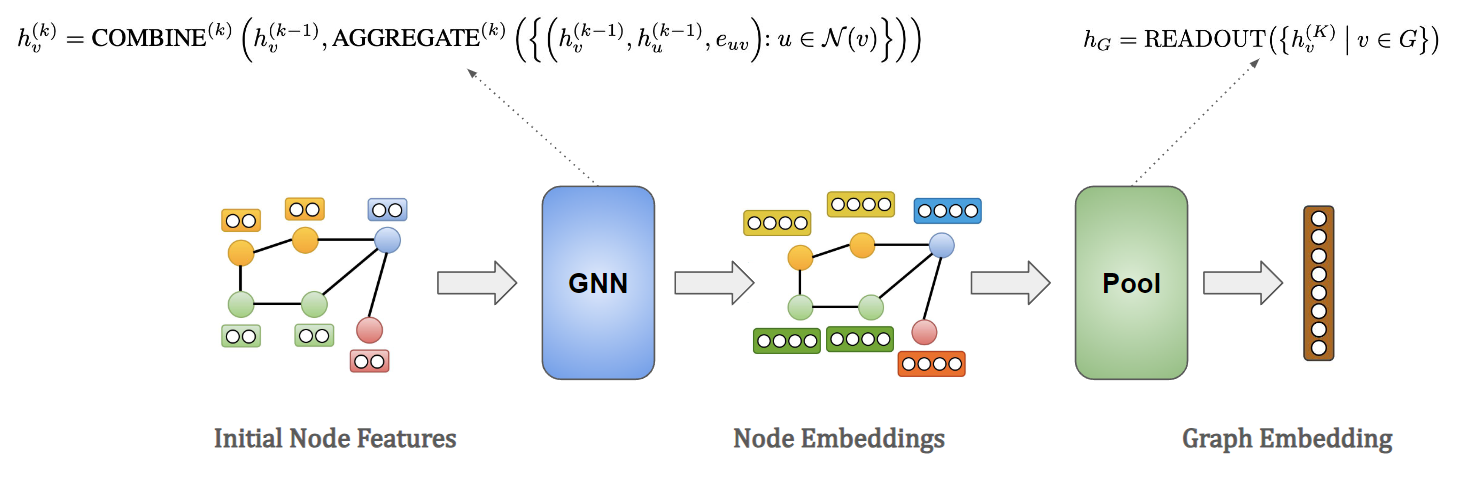
\includegraphics[width=1\linewidth]{Graphpooling.png}
    \caption{Read-out function}
    \label{fig:enter-label}
\end{figure}

\textbf{GNN Models}\\
\begin{itemize}
    \item Various ways of using aggregation functions lead to the creation of different Graph Neural Network (GNN) models.
\end{itemize}

\begin{figure}[h!t]
    \centering
    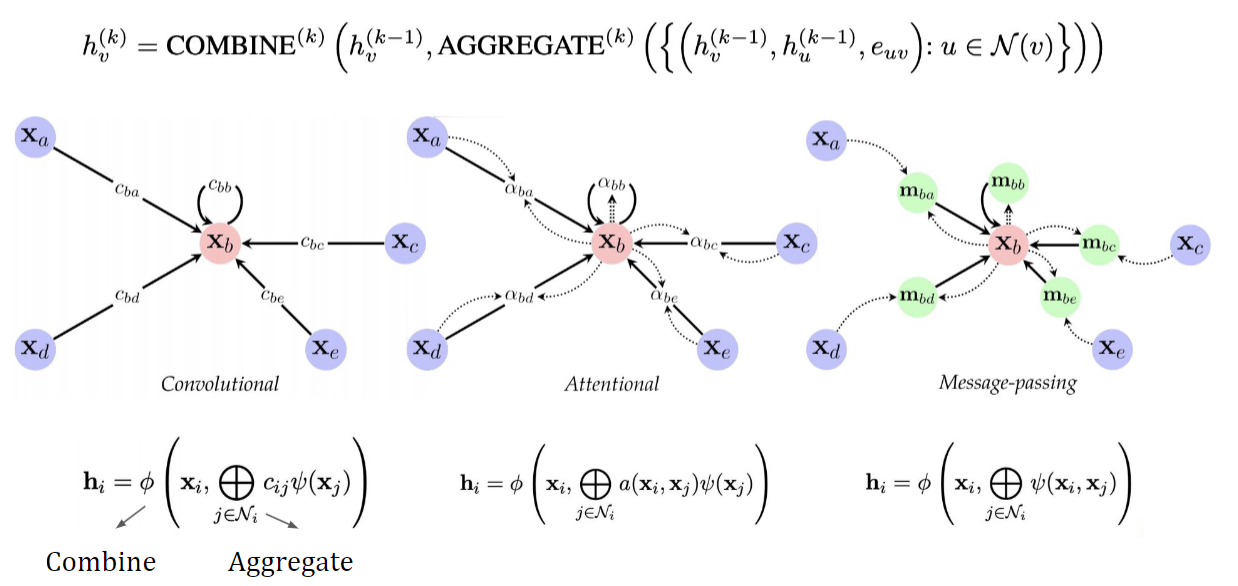
\includegraphics[width=1\linewidth]{gnnmodels.png}
    \caption{1.\textbf{ Convolutional}: Multiply importance of each neighbour by scalar and summing; \newline
    2. \textbf{Attentional}: Use attention mechanism to do weighted summation; 
    \newline
    3. \textbf{Message-Passing}: Pass all embeddings between target node and neighbouring nodes computed by neural network, then aggregate}
    \label{fig:enter-label}
\end{figure}

\section{Graph Convolutional Networks (GCNs)}

\begin{itemize}
    \item A layer of a GNN is basically a nonlinear function over node features and adjacency
matrix:
\[ H = f(A, X) \]
\item The simplest model we can define is:
\[ H = \sigma(AXW) \]
\begin{itemize}
    \item Where:
    \begin{itemize}
        \item  $\sigma$ is the non-linearity function
    \end{itemize}
    \begin{itemize}
        \item W is the weight matrix
    \end{itemize}
\end{itemize}
\item This is already a strong model, but has two limitations:

\end{itemize}
\begin{enumerate}
    \item Multiplication with A means that, for every node, we sum up all the feature vectors of all neighbouring nodes but not the node itself
    \begin{enumerate}
        \item Fix: Add self-loops (add the identity matrix to A) 
\[ A = A + I \]
    \end{enumerate}
    \item A is not normalized and therefore the multiplication with A will completely change the scale of the feature vectors
    \begin{enumerate}
        \item Fix: Symmetrically normalize A using diagonal degree matrix D such that all rows sum to one
\[ D^{-\frac{1}{2}}AD^{-\frac{1}{2}} \]

    \end{enumerate}
\end{enumerate}
\begin{itemize}
    \item With these fixes we define a GCN layer as follows:

\[ H = \sigma(D^{-\frac{1}{2}}AD^{-\frac{1}{2}}XW) \]


\end{itemize}

\textbf{Going Deeper}

\begin{itemize}
    \item A GCN layer updates the node embeddings based on the features of the immediate
neighbors (recall multiplication with A)
\item We can influence the embeddings from further neighborhood by stacking GCN layers
\item This is analogous to increasing the receptive field in CNNS
\end{itemize}

\begin{figure}[h!t]
    \centering
    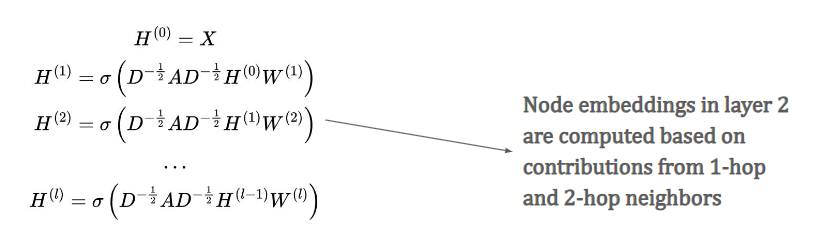
\includegraphics[width=0.75\linewidth]{stackingGCN.png}
    \caption{Stacking GCNs}
    \label{fig:enter-label}
\end{figure}

\section{Graph Attention Networks (GAT)}

\begin{idea}
    Instead of using node degree, learn an attention score between two nodes, i.e., learn the contribution weight of neighbor nodes
\end{idea}

\begin{enumerate}
    \item Use a shared neural network to compute an attention score between two nodes:
\[ e_{ij} = NN(h_i, h_j) \]
    \item Normalize the attention scores:
\[ \alpha_{ij} = softmax_j(e_{ij}) = \frac{exp(e_{ij})}{\sum_{k\in N_{i}}exp(e_{ik})} \]
    \item Update the node embeddings based on the attention score:

\[ h_i = \sigma(\sum_{j\in N_i} \alpha_{ij} W h_j) \]
\end{enumerate}

\section{PyTorch Implementation}
\begin{example}
    Suppose we want to classify the following molecule using a GCN to a toxic/non-toxic
where node features represent the atom type (Carbon, Hydrogen, Nitrogen).
\end{example}

\begin{figure}[h!t]
    \centering
    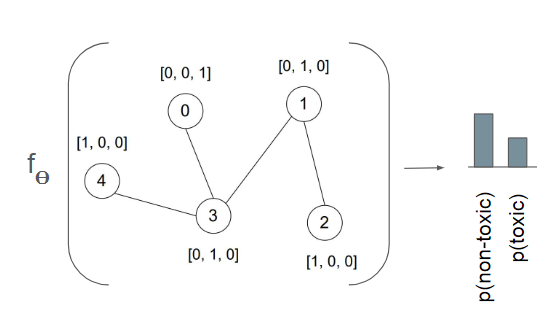
\includegraphics[width=0.7\linewidth]{toxicity.png}
    \caption{Toxicity classifier}
    \label{fig:enter-label}
\end{figure}

\noindent \textbf{Dense Implementation}

\begin{itemize}
    \item Most graphs are sparse
    \item Dense implementation uses $N^2$ space for adjacency
    \item We can represent this graph with only 4 edges where dense implementation represents it with 25
    \item Implementing sparse operations are supported by PyTorch but are not very straightforward
    \item We can use \textbf{PyTorch Geometric (PYG)}
\end{itemize}

\begin{figure}[h!t]
    \centering
    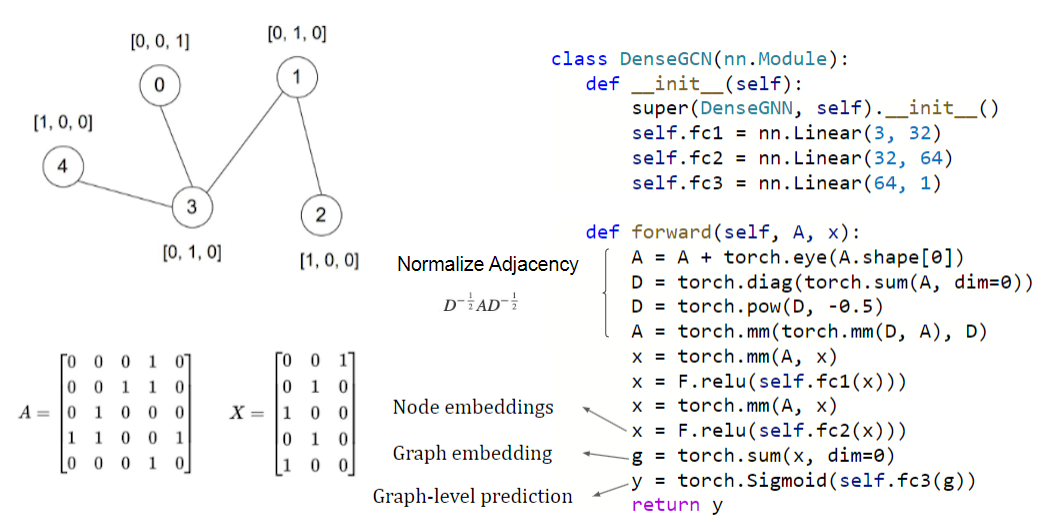
\includegraphics[width=1\linewidth]{denseimplementation.png}
    \caption{Dense Implementation}
    \label{fig:enter-label}
\end{figure}

\begin{figure}[h!t]
    \centering
    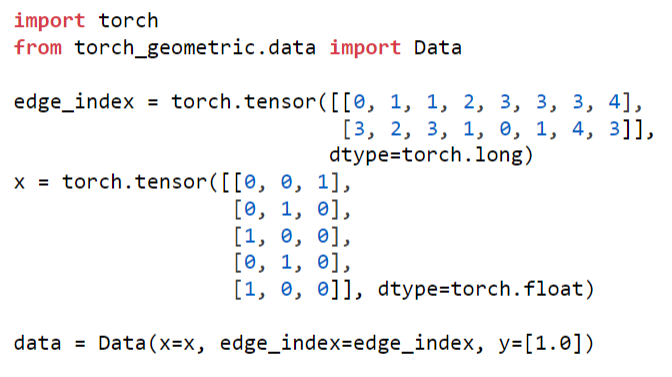
\includegraphics[width=0.75\linewidth]{sparseimp.png}
    \caption{Sparse implementation with PYG}
    \label{fig:enter-label}
\end{figure}

\newpage

\noindent \textbf{Sparse Implementation}

\begin{figure}[h!t]
    \centering
    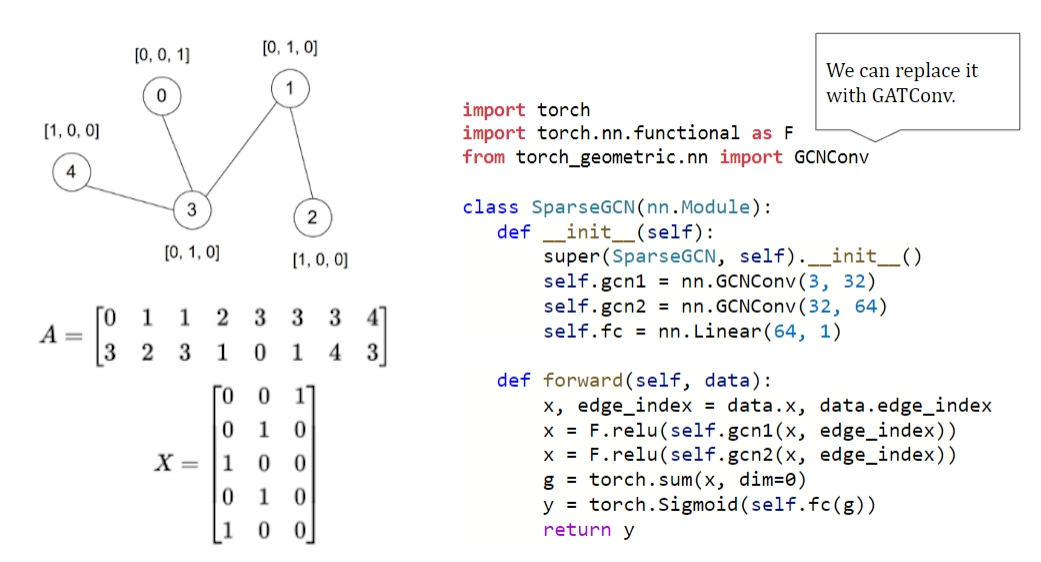
\includegraphics[width=1\linewidth]{sparseimplementation.png}
    \caption{Sparse Implementation}
    \label{fig:enter-label}
\end{figure}

Sparse implementation is better but dense implementation is more intuitive to implement.

\newpage

\noindent
\textbf{Dense vs. Sparse: Computational efficiency}\\
\begin{itemize}
    \item Dense GNNs assume dense connectivity and involve\textbf{ interactions between all nodes.}
    \item Sparse GNNs take advantage of the sparsity of the graph and \textbf{only consider interactions between connected nodes}, which is more efficient for sparsely connected graphs.
\end{itemize}

\textbf{Dense vs. Sparse: DataLoader \& Dataset}\\
\begin{itemize}
    \item Dense implementation: batching is done by creating a \textbf{diagonal matrix} of adjacency
matrices
\begin{itemize}
    \item Large scale graph datasets will almost always run out of memory
\end{itemize}

\begin{figure}[h!t]
    \centering
    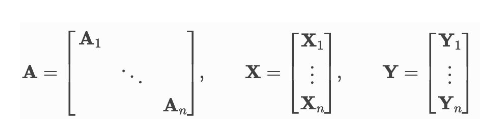
\includegraphics[width=0.75\linewidth]{dense.png}
    \caption{Batching in dense implementation}
    \label{fig:enter-label}
\end{figure}

\item Sparse implementation: uses an\textbf{ index vector} which maps each node to its respective
graph in the batch
\begin{itemize}
    \item Very simple and efficient
\end{itemize}
\end{itemize}

\begin{figure}[h!t]
    \centering
    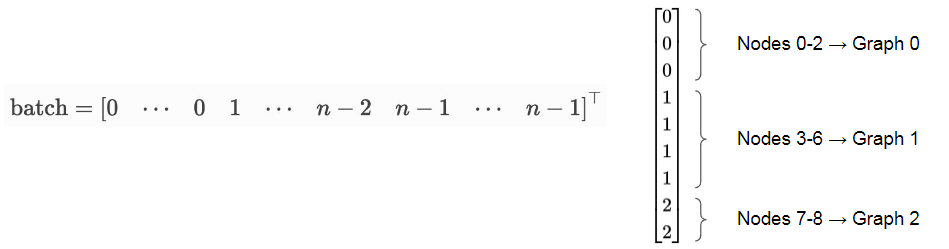
\includegraphics[width=1\linewidth]{sparse.png}
    \caption{Batching in sparse implementation}
    \label{fig:enter-label}
\end{figure}
\begin{figure}[h!t]
    \centering
    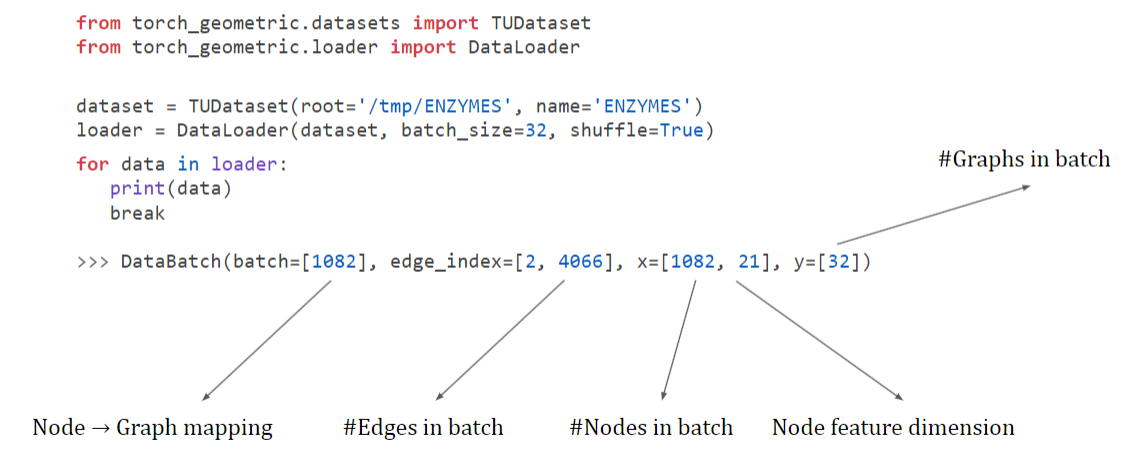
\includegraphics[width=1\linewidth]{dataset.png}
    \caption{Dataloader \& Dataset}
    \label{fig:enter-label}
\end{figure}